%!TEX root = ../dokumentation.tex
\chapter{Theory}

\section{Classification of Data}
%Data Types in ML (Cross-Sectional-, Time Series- and Panel Data)
Most data found in academic and industrial projects can be broadly classified into three categories:
\begin{itemize}
	\item Cross-sectional data
	\item Time series data
	\item Panel data
\end{itemize}

Cross-sectional data is data taken from multiple individuals at one point in time. The cross section of a population is obtained by taking observations from multiple individuals at the same time our without taking time into consideration at all. One example for this could be the test scores of all students for one particular exam. Another example is shown here:

\begin{figure}[ht]
	\centering
	\scalebox{1}{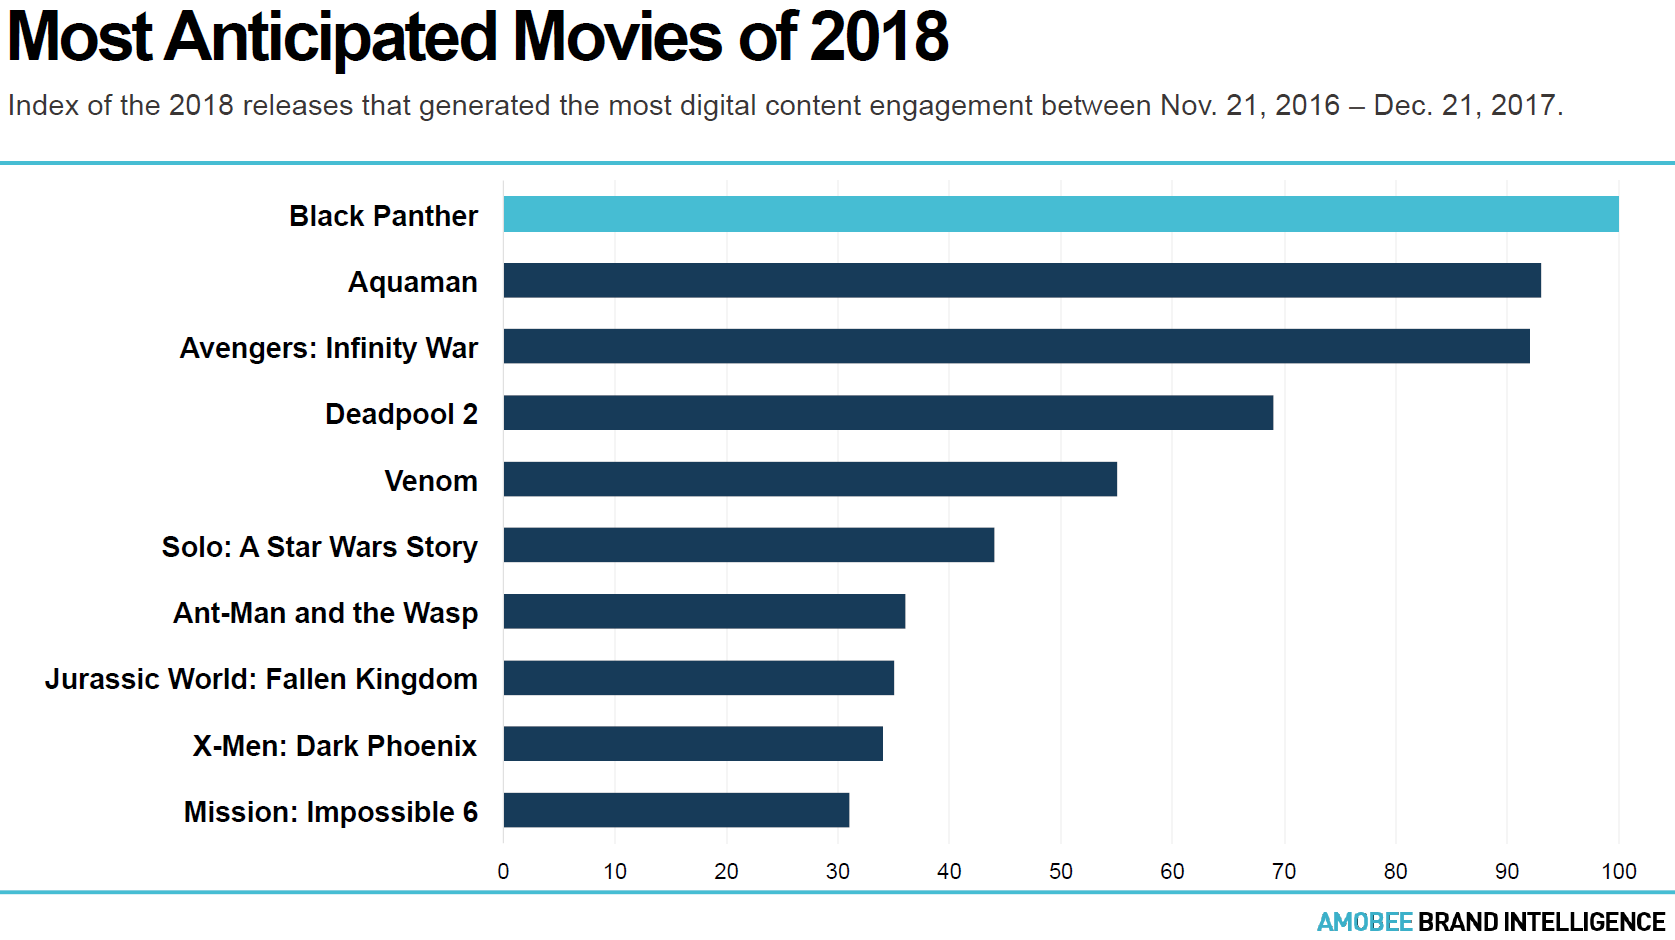
\includegraphics[width=0.475\textwidth]{images/example_cross-sectional_data.PNG}}%\scalebox{1}{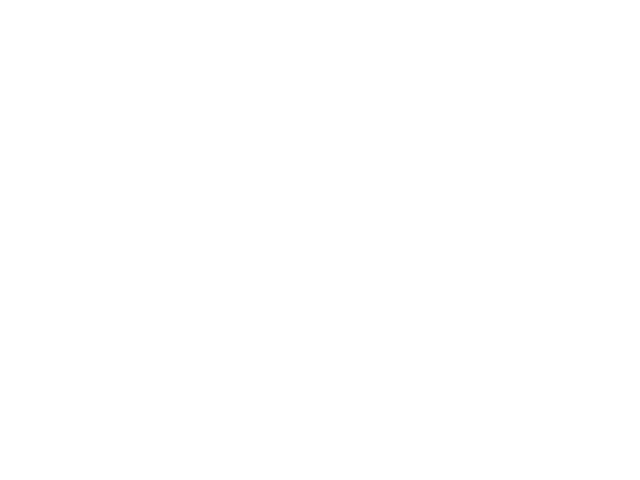
\includegraphics[width=05\textwidth]{images/empty-transparent.png}}\scalebox{1}{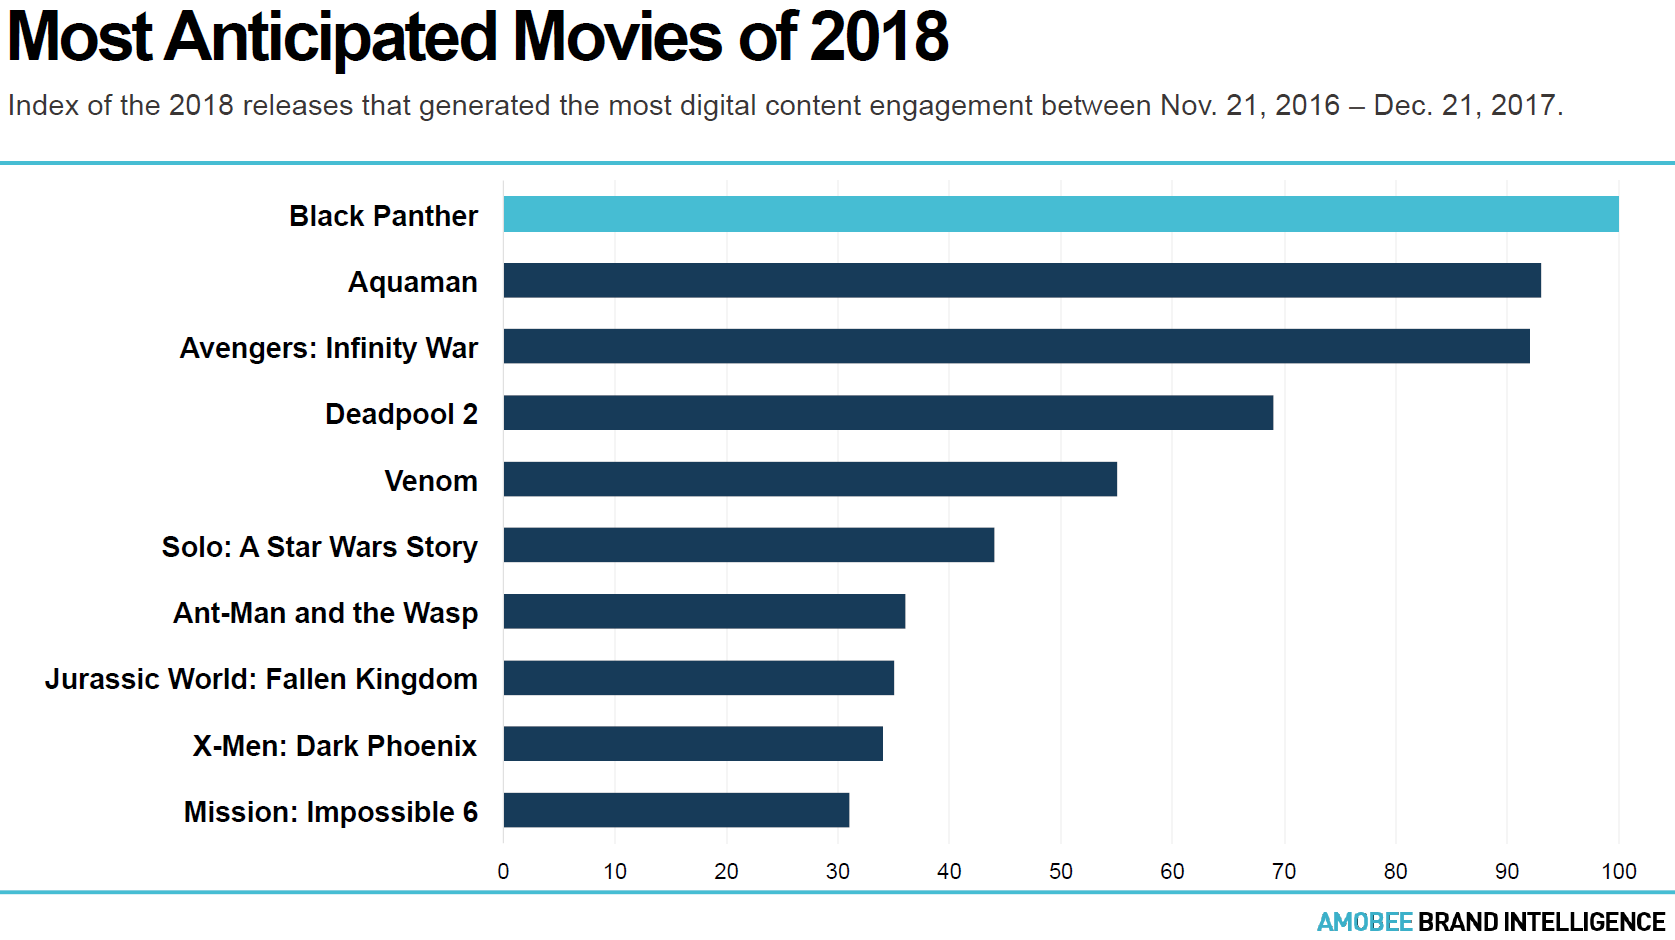
\includegraphics[width=0.475\textwidth]{images/example_cross-sectional_data.PNG}}
	\caption{Example for cross-sectional data \textsuperscript{\cite{-1}}}
\end{figure}

%https://www.cnbc.com/2018/02/16/black-panther-already-setting-records-with-thursday-box-office.html
%example_cross-sectional_data.PNG

Time series data is data taken from one individual at multiple points in time. A time series is made up of quantitative observations on one or more measurable characteristics of an individual entity and taken in an interval of time. The data is typically characterized by several internal structural elements such as trend, seasonality, stationarity, autocorrelation and noise. A common example for this would be sensor data, but also stock data when measured over time or the average income of politicians over the course of their career.

\begin{figure}[ht]
	\centering
	\scalebox{1}{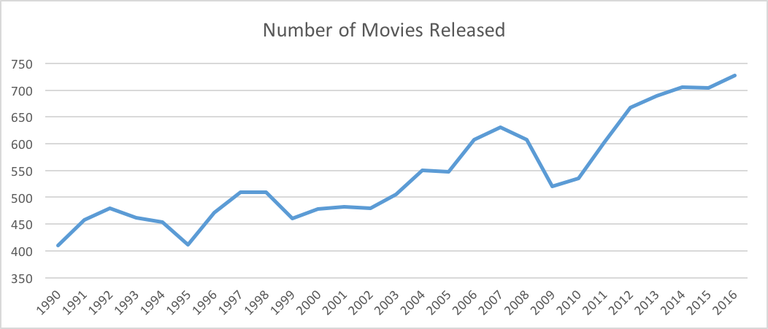
\includegraphics[width=0.475\textwidth]{images/example_timeseries_data.PNG}}
	\caption{Example for time series data \textsuperscript{\cite{-1}}}
\end{figure}

The last category is a combination of the first two. Panel Data can be defined as data taken from multiple individuals at multiple points in time and also known as longitudinal data.

An example for panel data would be Military Expenses of all European countries from 2001 to 2010. And one of the methods used to analyses this type of dataset is called “fixed effects model” which itself is also type of regression model.

\begin{figure}[ht]
	\centering
	\scalebox{1}{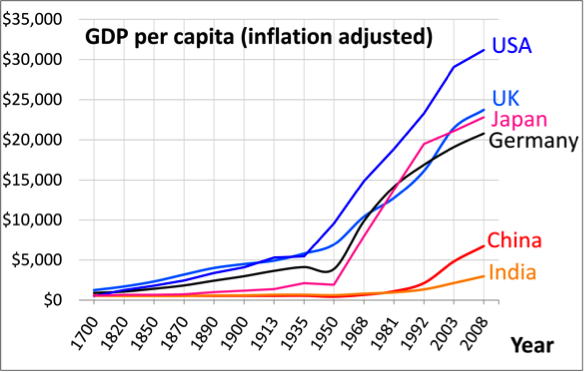
\includegraphics[width=0.475\textwidth]{images/example_panel_data.PNG}}
	\caption{Example for panel data \textsuperscript{\cite{-1}}}
\end{figure}

Methods for analyzing any of this data include plotting of variables to visualize statistical properties and calculation of central tendency, variance, skewness, and kurtosis. 

%\pagebreak
\section{Time Series Analysis}

Analyzing time series is about understanding and modeling the different characteristics that time series data can exhibit. The most commonly studied features of time series data are:
\begin{itemize}
	\item Noise
	\item General trend
	\item Cyclic movements
	\item Seasonality
	\item Pulses and Steps
	%\item Outliers
	\item Stationarity
\end{itemize}

The first one that is mostly referred to as \textit{noise} reflects unexpected variations in the time series. It is often used to describe a type of error in a time series model that is due to a lack of information about explanatory variables that can model these variations or due to presence of random noise.

And there can be different models used in which there is no trend nor seasonal component. One of the those models describes the \acl{iid} noise or \acs{iid} noise. In this model observations are simply \acl{iid} variables with zero mean and it is also called white noise. This means that this model doesn't not have dependencies between observations.

However there is also another model that does show dependencies. And it is know as \textit{Random Walk Model}. The random walk \(S_t \) obtained by cumulatively summing \acs{iid} random variables \([Z_t]\) with \(S_0=0\) and can therefore be defined as:

\begin{equation}\label{eq:random_walk_model}
	S_t = Z_1 + Z_2 + Z_3 + ... + Z_t
\end{equation}

If furthermore the random variables \([Z_t] \) are Bernoulli distributed with \(p=0.5\) then this is called a simple symmetric random walk. An example for this could be a pedestrian who starts a position zero at time zero and at each integer time tosses a fair coin, stepping one unit to the right each time a head appears and one unit to the left for each tail. Both these model are referenced to as \textit{zero-mean models}.
An example of the random walk model as well as an \acs{iid} model can be seen in Figure 2.4.

\begin{figure}[ht]
	\centering
	\scalebox{1}{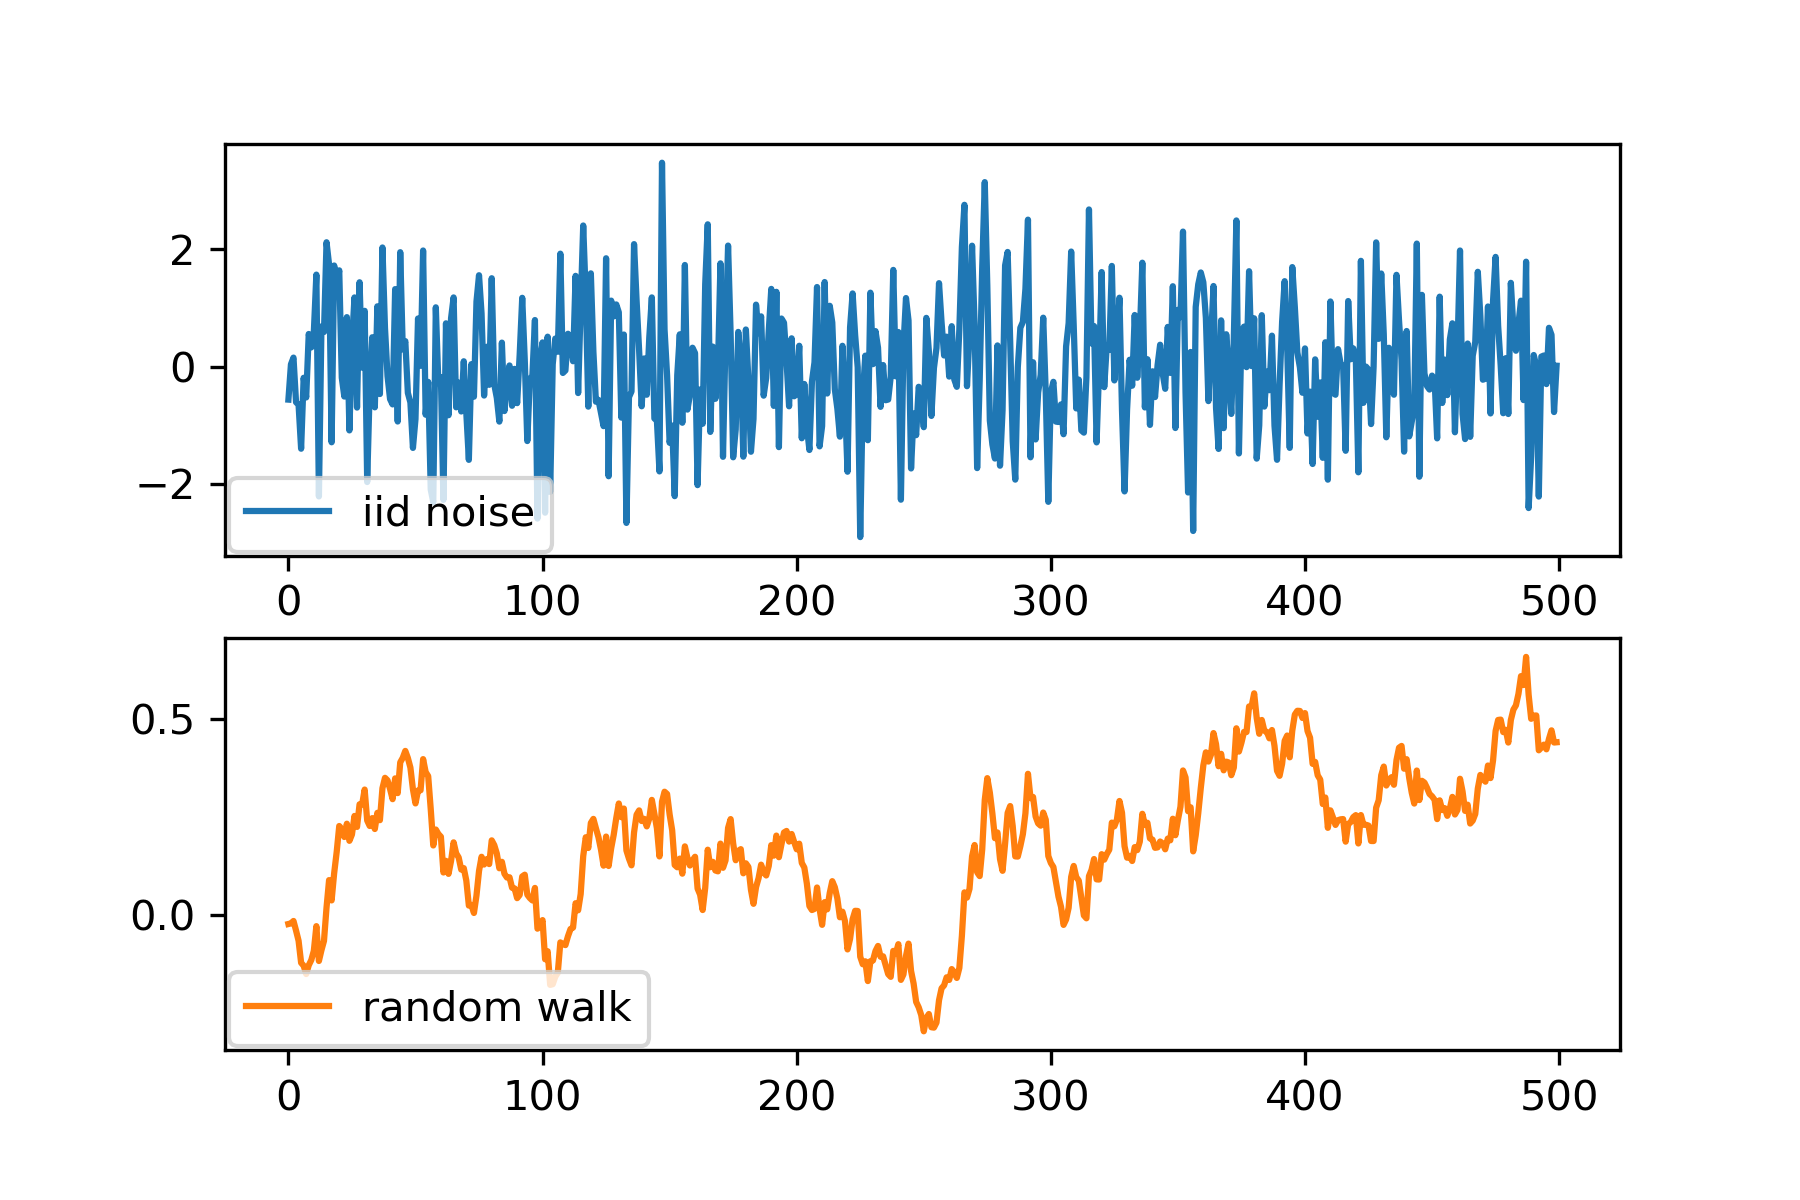
\includegraphics[width=0.66\textwidth]{images/example_noise.png}}
	\caption{Example for iid model (top) and random walk model (bottom)}
\end{figure}

In several time series there is also a clear trend to be observed in the data. This means it exhibits an upward or downward movement in the long run. In those cases a zero mean model is not sufficient to describe the series. 
Trend models aim to capture this long run trend in a time series. They can be fitted as linear regressions of the time index. And for this a trend model \(X_t\) can be expresses as the sum of the trend component \(m_t\) being a slowly changing function and a zero mean model \(z_t\):

\begin{equation}\label{eq:simple_trend_model}
	X_t = m_t + z_t
\end{equation}

\begin{figure}[ht]
	\centering
	\scalebox{1}{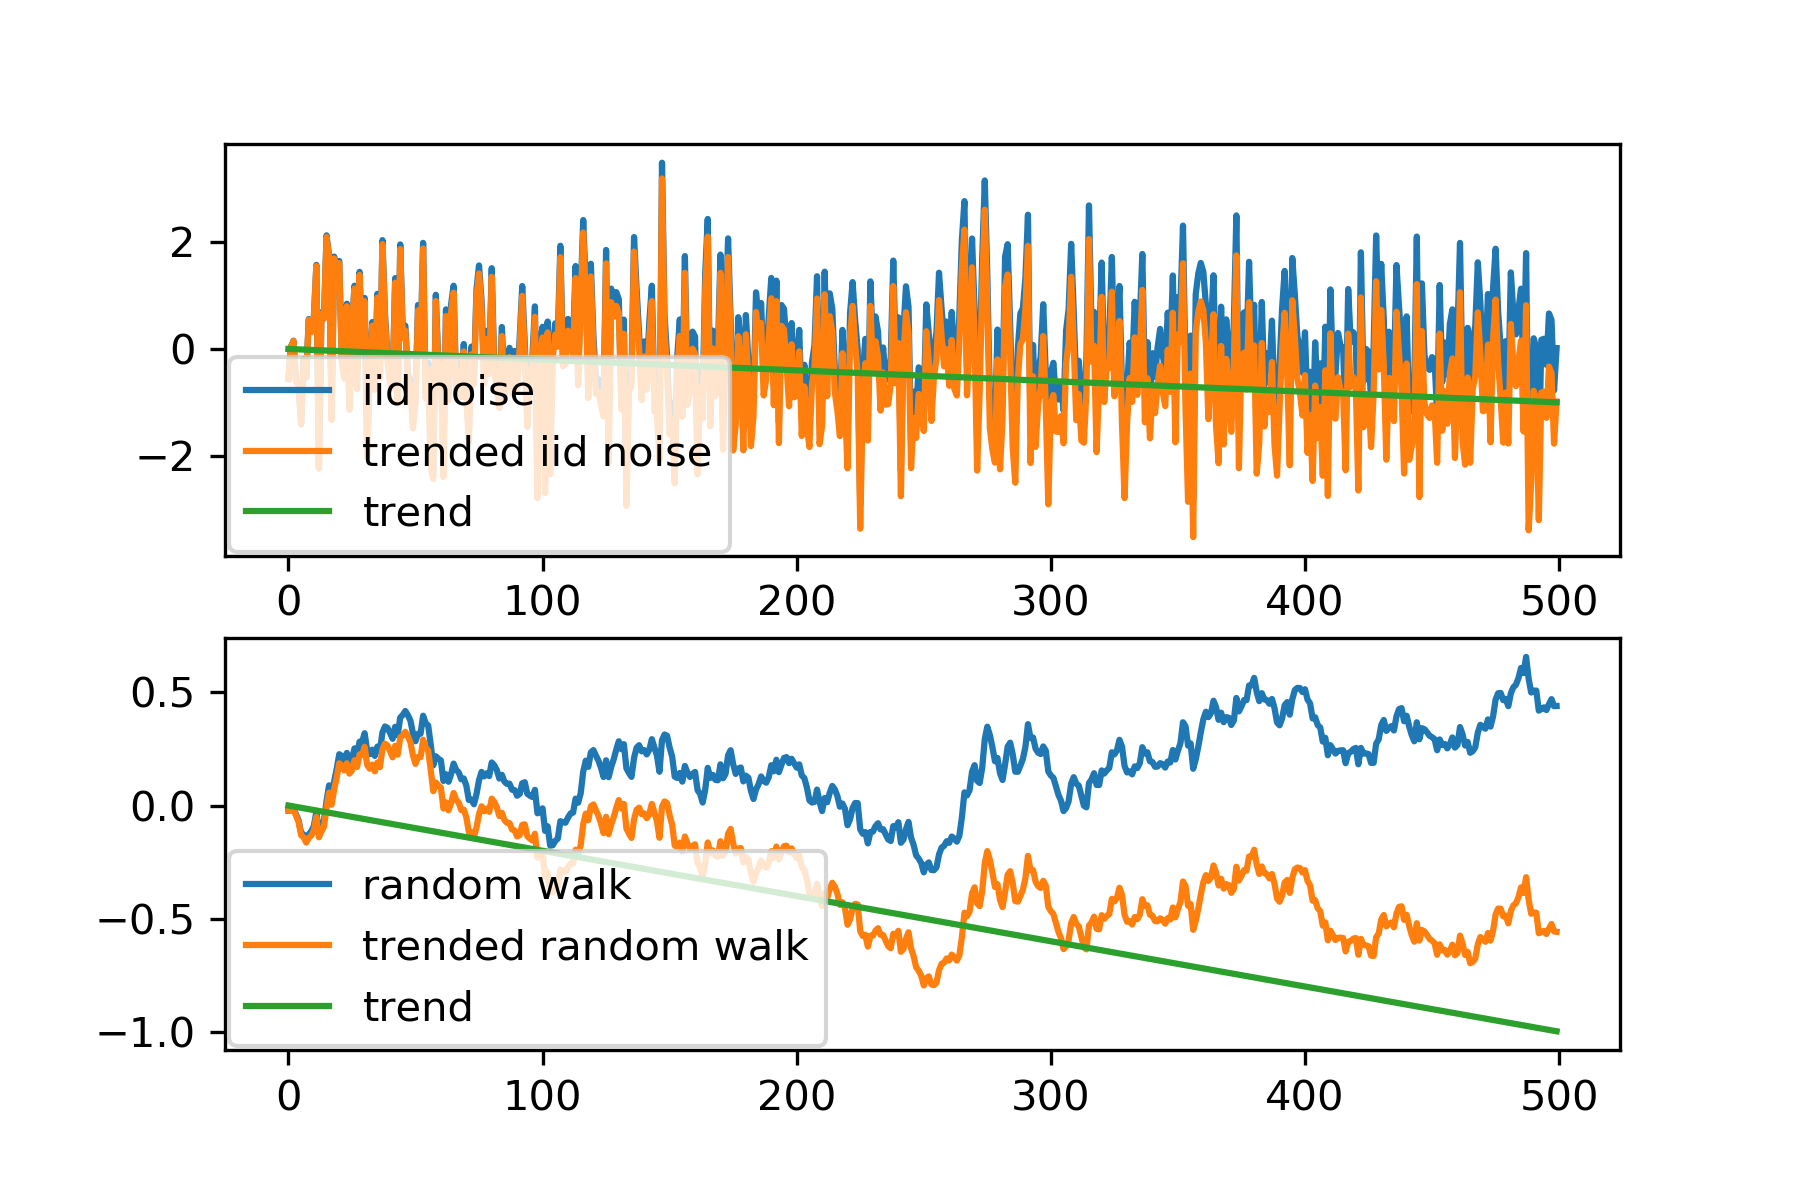
\includegraphics[width=0.66\textwidth]{images/example_trendednoise.png}}
	\caption{Example of trend models using  \acs{iid} and random walk as zero mean models}
\end{figure}

Besides general trend and noise many time series are also influenced by factors that occurs periodically. These repetitive fluctuations are called \textit{cyclic movements}. These can further be divided into nonseasonal cycles and seasonal cycles.

Nonseasonal cycles are repetitive, possibly unpredictable patterns in time series values and defined by a periodicity that varies of time. 

In contrast to that, seasonal cycles have a known \textbf{constant} periodicity. And in that case the time series is to be said to exhibit seasonality.  One example causing seasonality in a series is dependency of the observed system on  weather. It itself is seasonal and when the weather then interferes with the observed system this interference can be seen in periodic fluctuations that occurs in a fixed period.

%2002 Brockwell, Introduction to Time Series and Forecasting
In order to represent such seasonal effects, allowing for noise but assuming no trend, we can use a model that can be expressed as combination of an harmonic regression and the zero mean model 

\begin{equation}\label{eq:simple_seasonal_model}
	X_t = s_t + z_t
\end{equation}
where \(s_t\) is a periodic function of t with period d (\(s_{t-d}= s_t\)) and is defined as: 


\begin{equation}\label{eq:harmonic_regression}
	s_t = a_0 + \displaystyle\sum_{j=1}^{k} (a_j \cos(\lambda t) + b_j \sin(\lambda t ))
\end{equation}

here \(a_0, a_1, . . . , a_k\) and \(b_1, . . . , b_k\) are unknown parameters and \(\lambda_1, . . . , \lambda_k\) are fixed frequencies, each being some integer multiple of \(2\pi/d\).

\begin{figure}[ht]
	\centering
	\scalebox{1}{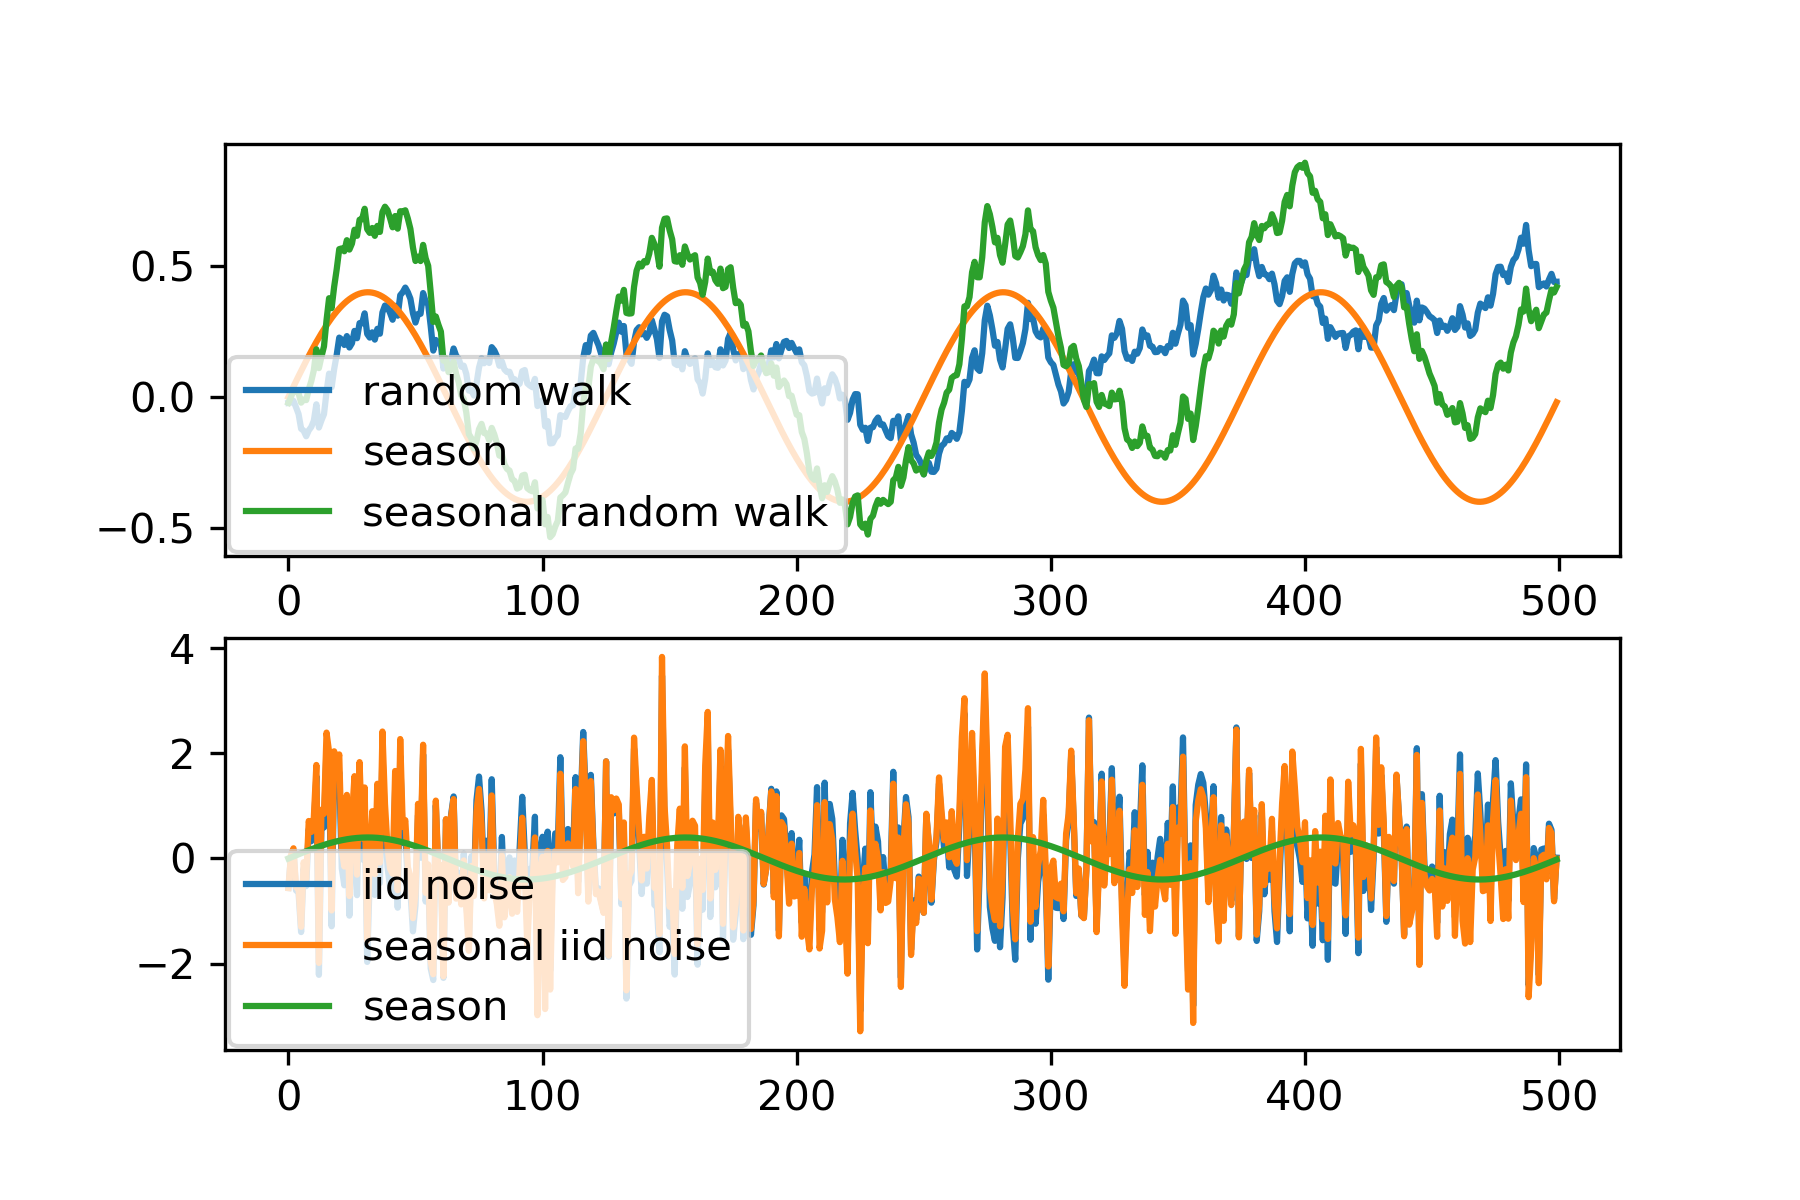
\includegraphics[width=0.66\textwidth]{images/example_season_and_noise.png}}
	\caption{Example of seasonal models using \acs{iid} and random walk as zero mean models}
\end{figure}

By using an additive model \(X_t= m_t + s_t + z_t\) combining a trend component \(m_t\), a seasonal component \(s_t\) and the random walk model as the noise or zero-mean component \(z_t\) a time series can be decomposed and visually represented like in figure 2.6. However real time series data is usually not that easily modeled, because they usually also show other more complex characteristics that are harder to model and therefore predict. These include \textit{pulses} and \textit{steps} as well as different types of \textit{outliers}.

\begin{figure}[ht]
	\centering
	\scalebox{1}{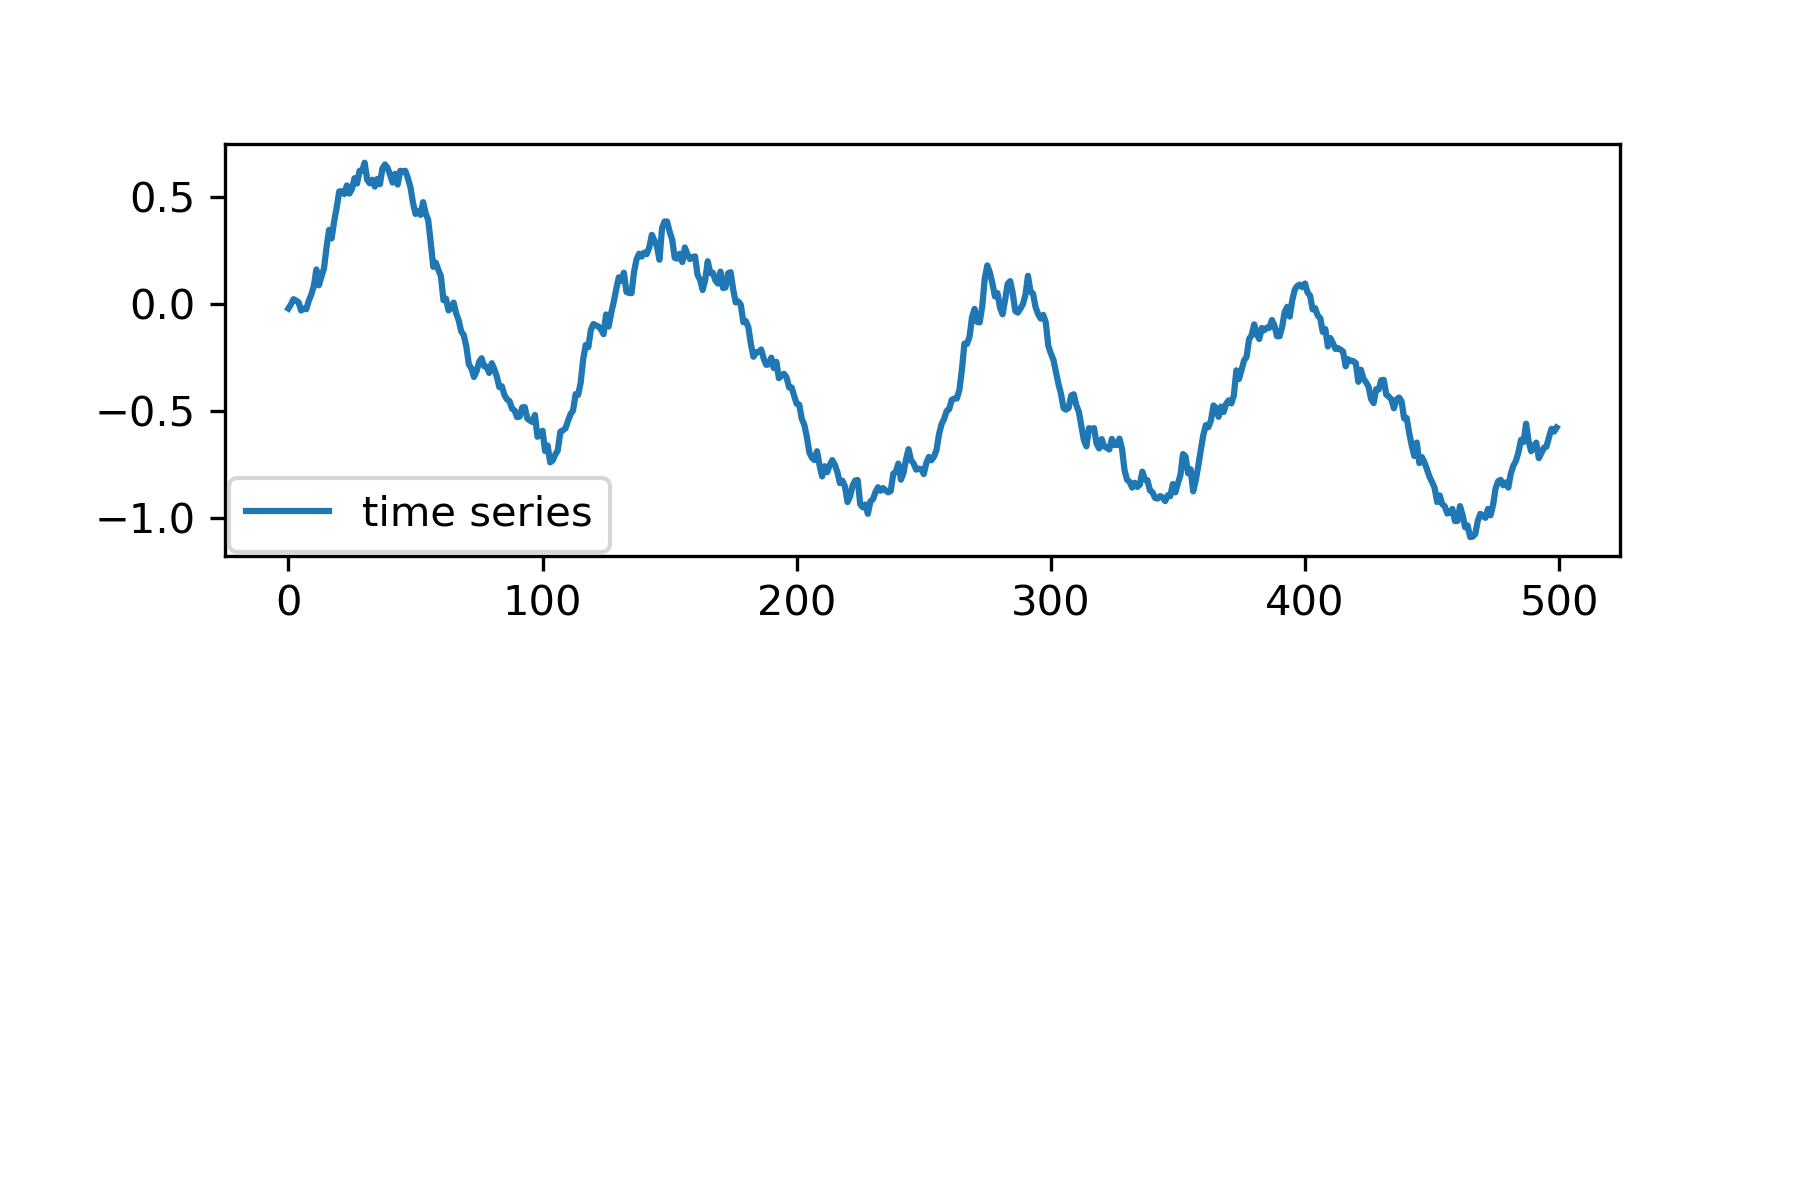
\includegraphics[width=0.6\textwidth]{images/example_timeseries_characteristics.png}}
	\caption{Example of time series decomposed into seasonal, trending and zero mean model}
\end{figure}
\textit{Pulses} and \textit{steps} are abrupt changes in level that a series might exhibit:
A \textit{pulse} is defined as a temporary shift and a \textit{step} is a permanent shift in the series.

%"":
When steps or pulses are observed, it is important to find a plausible explanation. Time series models are designed to account for gradual, not sudden, change. As a result, they tend to underestimate pulses and be ruined by steps, which leads to poor model fits and uncertain forecasts. If a disturbance can be explained, it can be modeled using an intervention or event. 
%https://www.ibm.com/support/knowledgecenter/SS3RA7_17/components/dt/timeseries_pulses.html?view=embed

\begin{figure}[ht]
	\centering
	\scalebox{1}{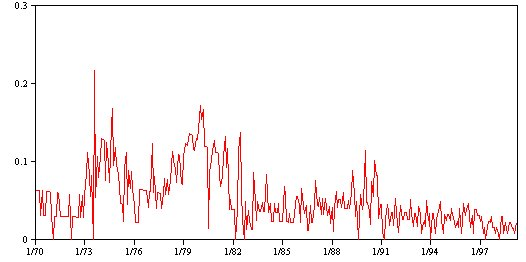
\includegraphics[width=0.66\textwidth]{images/example_pulse.jpg}}
	\caption{Example of a pulse in a time series}
\end{figure}

%if not enough pages add outliers: https://www.ibm.com/support/knowledgecenter/SS3RA7_17/components/dt/ts_outliers_overview.html

%https://people.duke.edu/~rnau/411diff.htm
%https://pdfs.semanticscholar.org/0f08/bcca67b3db328edfa5d3f48331dc71d8789e.pdf
%2002 Brockwell, Introduction to Time Series and Forecasting
A particular importance to many time series forecasting models has the characteristic that is called stationarity. This is because a lot of time series models use the assumption that the series to be forecast is already stationarity or can be made approximately stationary through the means of mathematical transformations. 
A time series is called stationary if its statistical properties stay constant over time. These restrictions only have to apply to those properties that depend only on the first- and second-order moments of \(X_t\):

Let \({X_t}\) be a time series with \(E(X_t^2 ) < \infty\). The mean function of \({X_t }\) is

\begin{equation}\label{eq:mean_function}
	\mu_X(t) = E(X_t )
\end{equation}
The covariance function of \({X_t }\) is

\begin{equation}\label{eq:covariance_function}
	\gamma_X(r, s)  = Cov(X_r,X_s)  E[(X_r - \mu_X(r))(X_s - \mu_X(s))]
\end{equation}
for all integers r and s.
\({X_t }\) is (weakly) stationary if
\begin{enumerate}
\item [i] \(\mu_X(t)\) is independent of t,
\item [and]
\item [ii] \(\gamma_X(t + h, t) \) is independent of t for each h.
\end{enumerate}

%https://people.duke.edu/~rnau/411diff.htm
To obtain meaningful statistical properties such as mean, variance, and correlations a timer series has to be stationarized first. Only then such statistics can be used as descriptors for future behavior.
For example, if the series is consistently increasing over time, the sample mean and variance will grow with the size of the sample, and they will always underestimate the mean and variance in future periods. And therefore based on the mean and variance the correlation with other variables would be under- or overestimated too.

This is why there is a need for mathematical transformations that can make a non-stationary time series approximately stationary.

One of those mathematical transformations is called \textit{de-trending} and can be used when the series has a stable long-run trend and no seasonality. This is achieved by fitting a trend model to the time series and then subtracting it from the original series. The resulting time series can then be further analyzed and modeled and is called \textit{trend-stationary} if the process was able to stationarize the series. An equivalent process is working for time series which do show seasonality. Of course in those cases a seasonal model has to be fitted and then subtracted from the series. There is also the possibility of combining both of those approaches.

However, not all time series can be stationarized by these processes. For some series this is insufficient and they might have to be differenced, either from period to period or from season to season. The idea is that if, even after removing a trend and/or seasonal model, the statistical characteristics are still not constant over time, then the statistics of the changes in the series between periods or seasons might be constant. In that case it is said to be \textit{difference-stationary}. Using unit-root tests can help identifying what stationarizing method might be more successful.

For the process of nonseasonal \textit{first order differencing} the \textit{lag-1} operator \(\Delta\) is defined by:

\begin{equation}\label{eq:seasonal_first_difference}
	\Delta X_t = X_t - X_{t-1} = (1-B)X_t
\end{equation}

where B is the backward shift or \textit{backshift} operator

\begin{equation}\label{eq:bachshift_operator}
	B X_t = X_{t-1}
\end{equation}

Powers of operators \(B\) and \(\Delta\) are defined by \(B^j X_t = X_{t-j}\) and \(\Delta^j X_t = \Delta (\Delta^{j-1} X_t), j >= 1\) with \(\Delta^0 X_t = X_t\). Polynomials in \(B\) and \(\Delta\) are manipulated in precisely the same way as polynomial functions of real variables. For example:

\begin{equation}\label{eq:example_delta_squared}
	\Delta^2 X_t = \Delta (\Delta X_t) = (1-B)(1-B)X_t = (1-2B + B^2) X_t = X_t - 2 X_{t-1} +  X_{t-2}
\end{equation}

\begin{figure}[ht]
	\centering
	\scalebox{1}{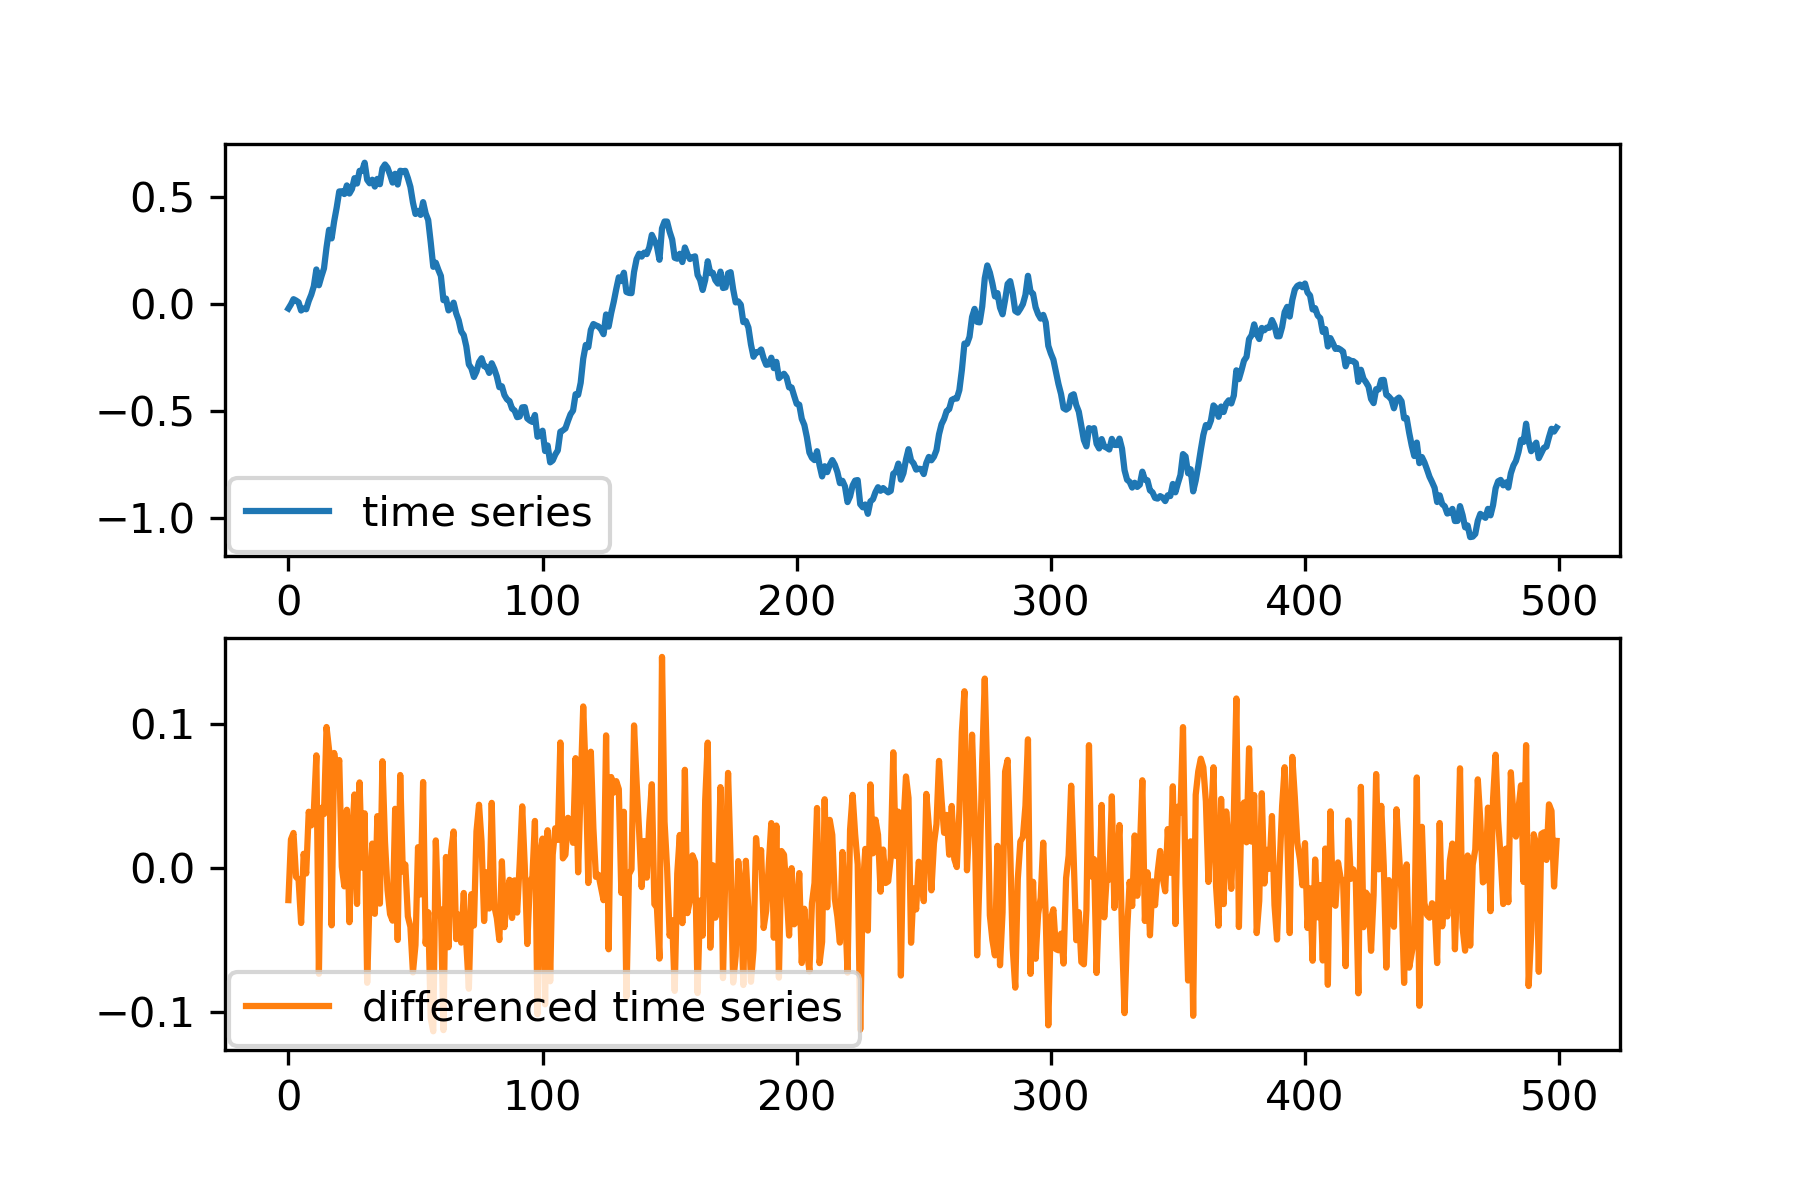
\includegraphics[width=0.66\textwidth]{images/example_firstorderdiff.png}}
	\caption{Example of a time series with its first order non-seasonal difference}
  \label{fig:example_non_seasonal_diff}
\end{figure}

\textit{First order differencing} is an example for a period to period differencing and is used to removed the trend from a time series. However, as seen in \ref{fig:example_non_seasonal_diff} the seasonality is still exhibited in the same way and to remove this as well seasonal differencing as to be applied additionally.

For the process of seasonal \textit{first order differencing} the \textit{lag-1} operator \(\Delta_s\) with seasonality \(s\) is defined by:

\begin{equation}\label{eq:seasonal_first_difference}
	\Delta_s X_t = X_t - X_{t-s} = (1-B^s)X_t
\end{equation}

And the \textit{D-th order difference} is defined by:

\begin{equation}\label{eq:seasonal_first_difference}
	\Delta_s^D X_t = (X_t - X_{t-s})^D = (1-B^s)^DX_t
\end{equation}

\begin{figure}[ht]
	\centering
	\scalebox{1}{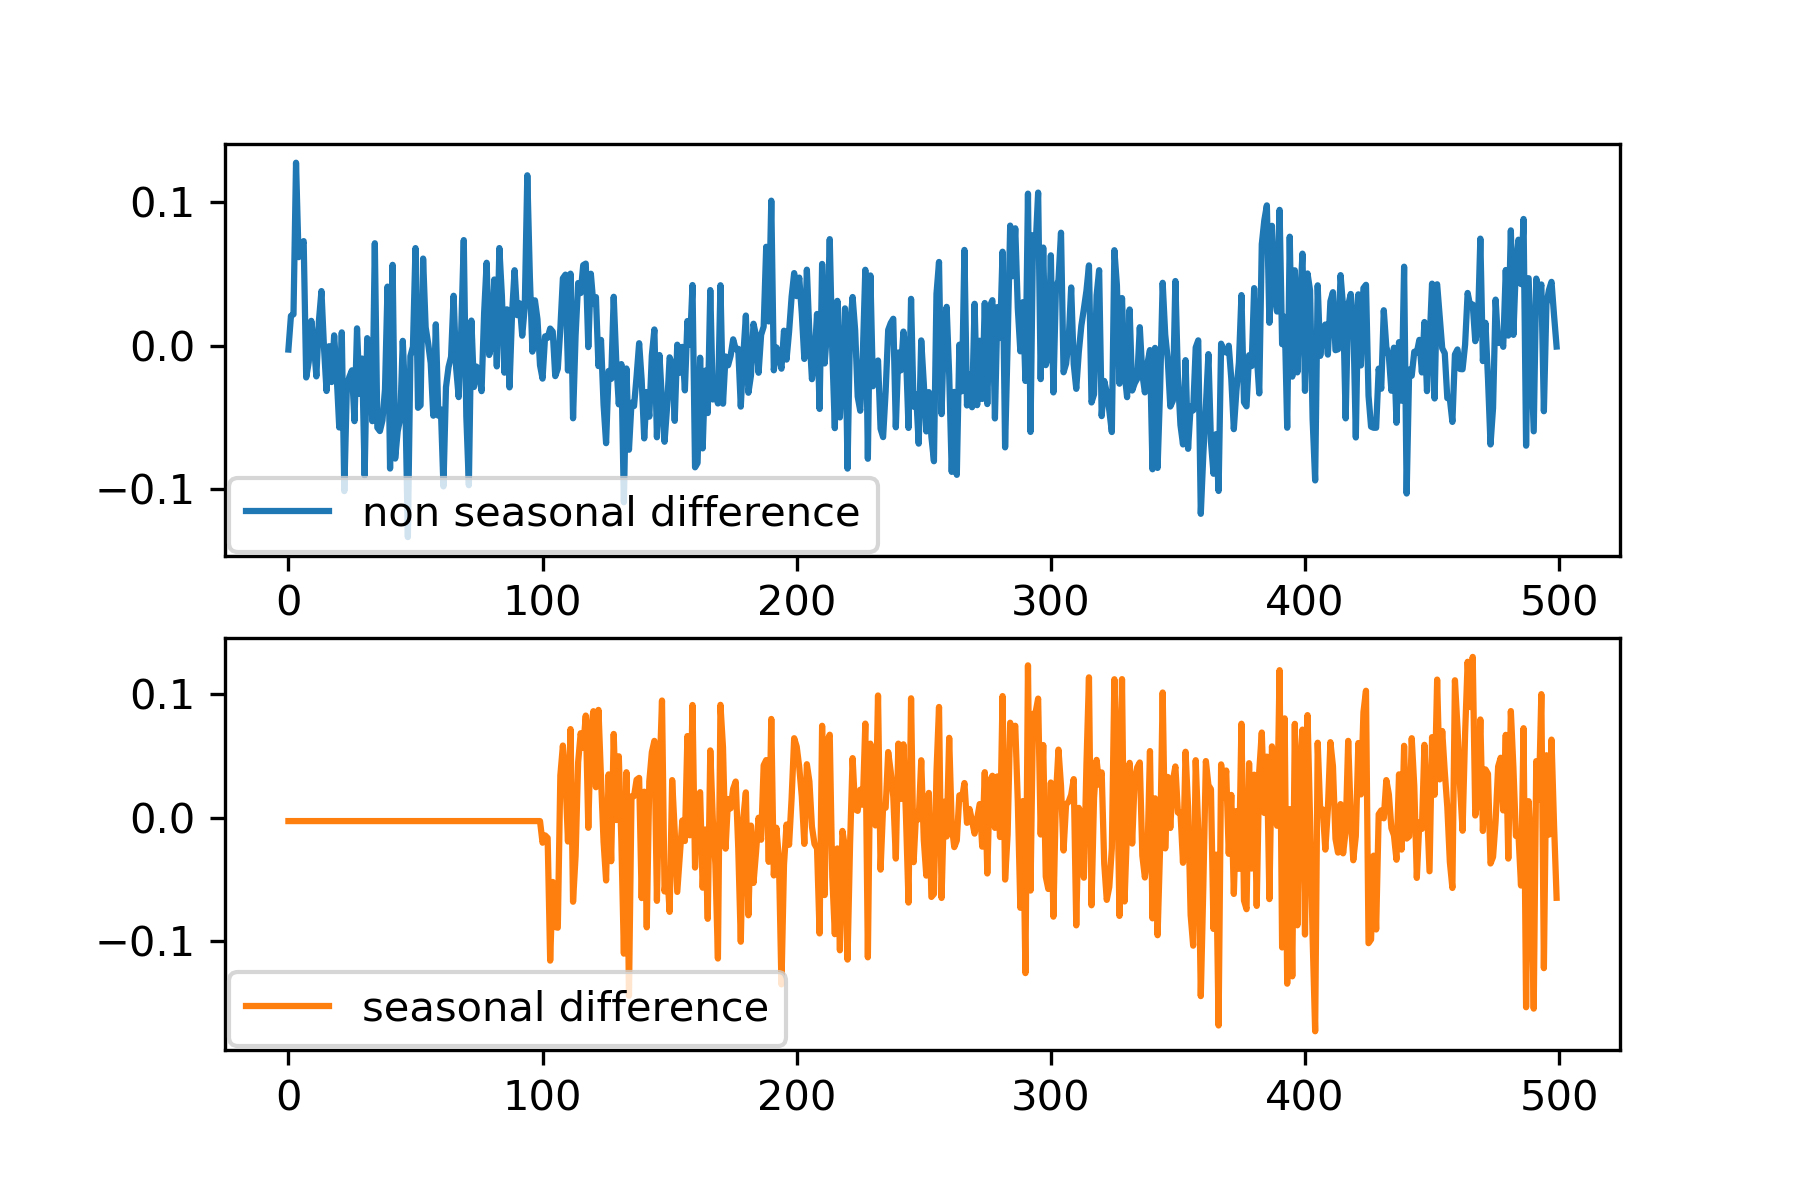
\includegraphics[width=0.66\textwidth]{images/example_seasonaldiff.png}}
	\caption{Example of a time series with its first order non-seasonal difference}
  \label{fig:example_seasonal_diff}
\end{figure}

%Characteristics of Time Series Data and how to model them
%Smoothing
%Smoothing is often referred to as filtering.
%There are two distinct groups of smoothing methods
%- Averaging Methods (Moving Average)
%- Exponential Smoothing Methods
%Autocovariance and (Partial) Autocorrelation


\section{ARIMA Model}
The \acs{ARIMA} (\acs{ARIMA}) model is used to better understand and forecast time series data. It is based on the \acs{ARMA} model but can also handle data that shows evidence of non-stationarity.  
\acs{ARMA} is composed out of the \acl{AR} (\acs{AR}) model and the \acl{MA} (\acs{MA}) model.

\acl{AR} models are used to predict future values of a time series by using linear combinations of previous values of the series and \acl{MA} models try to forecast by combining the prediction error that has been made for previous predictions in the time series.

Given a univariate time series \(X_t\) that is stationary and \(e_t\) a random variable with an independent and identical distribution representing the error that can occur in any prediction, the \acs{AR}\((p)\) model is defined by:
\begin{equation}\label{eq:AR_p}
	X_t = e_t + \displaystyle\sum_{i=1}^{p} (\phi_i B^i) X_t = e_t + \phi_1 X_{t-1}+ \phi_2 X_{t-2}+ ... + \phi_p X_{t-p}
\end{equation}

By defining the error of a prediction as the difference between the correct value from the time series and the value from the approximation \(\hat{X_t}\) as: 

\begin{equation}\label{eq:error_term}
	e_t = X_t - \hat{X_t}
\end{equation}

The approximation of \(X_t\) using an \acs{AR}\((4)\) can be written as:

\begin{equation}\label{eq:AR_four}
  \hat{X_t} = \phi_1 X_{t-1}+ \phi_2 X_{t-2}+ \phi_3 X_{t-3}+ \phi_4 X_{t-4}
\end{equation}

The \acl{MA} model is based on the definition \eqref{eq:error_term} of the error term \(e_t\). In contrast to the \acs{AR} model it combines \(e_t\) terms instead of just combining\(X_t\). Hence the definition of \acs{MA}\((q)\) is:

\begin{equation}\label{eq:MA_q}
	X_t = e_t + \displaystyle\sum_{k=1}^{q} (\theta_k B^k) e_t = e_t + \theta_1 e_{t-1}+ \theta_2 e_{t-2}+ ... + \theta_p e_{t-q}
\end{equation}

This makes the calculation of an \acs{MA}\((q)\) model a little bit more complicated, as demonstrated on the example of \acs{MA}\((3)\):

\begin{equation}\label{eq:example_MA_three_1}
	X_t = e_t + \theta_1 e_{t-1}+ \theta_2 e_{t-2} + \theta_3 e_{t-3}
\end{equation}

Replacing \(e_t\) with its definition \eqref{eq:error_term} and transforming the equation to \(\hat{X_t}\) makes the complication clearer:

\begin{equation}\label{eq:example_MA_three_2}
	\hat{X_t} =\theta_1 (X_{t-1} - {\hat{X}}_{t-1}) + \theta_2 (X_{t-2} - {\hat{X}}_{t-2}) + \theta_3 (X_{t-3} - {\hat{X}}_{t-3})
\end{equation}

In this form it is clear that \(\hat{X_t}\) is depended on \({\hat{X}}_{t-1}\), \({\hat{X}}_{t-2}\), \({\hat{X}}_{t-3}\) which are also unknown variables that have to be calculated first. Using the same formula for \({\hat{X}}_{t-1}\) and so on, this leads to more dependencies which lead to even more. What one eventually ends up with is a system of linear equation that, assuming \(X_t\) is a series of length 5 looks like this: 

\begin{equation}\label{eq:example_MA_three_system_1}
  \begin{array}{lcl}
    {\hat{X}}_{5} & = & \theta_1 (X_{4} - {\hat{X}}_{4}) + \theta_2 (X_{3} - {\hat{X}}_{3}) + \theta_3 (X_{2} - {\hat{X}}_{2}) \\
    {\hat{X}}_{4} & = & \theta_1 (X_{3} - {\hat{X}}_{3}) + \theta_2 (X_{2} - {\hat{X}}_{2}) + \theta_3 (X_{1} - {\hat{X}}_{1}) \\
  {\hat{X}}_{3} & = & \theta_1 (X_{2} - {\hat{X}}_{2}) + \theta_2 (X_{1} - {\hat{X}}_{1})\\
  {\hat{X}}_{2} & = & \theta_1 (X_{1} - {\hat{X}}_{1})\\
  {\hat{X}}_{1} & = & 0
  \end{array}
\end{equation}

To be able to calculate this for larger time series, some kind of solving mechanism is needed. To be able to use one of those the system of linear equations needs to be in the form of:

\begin{equation}\label{eq:syslinequation}
	 \mathbf{A}  \vec{\hat{x}} = \vec{b}
\end{equation}

with $\mathbf{A} \in \mathbb{R}^{n\times n}$ being a $n\times n$ Matrix,  $\vec{\hat{x}} \in \mathbb{R}^n$ and  $\vec{b}\in \mathbb{R}^n$ both vectors. The vector of $\vec{b}$ representing the known values for each equation, $\vec{\hat{x}}$ the unknown variables and $\mathbf{A}$ the coefficients of all the $\vec{\hat{x}}$ for each equation.

To see how $\mathbf{A}$ and  $\vec{b}$ have to be constructed the system of linear equations \eqref{eq:example_MA_three_system_1} can be transformed to:
\begin{equation}\label{eq:example_MA_three_system_2}
  \begin{array}{rcrcrcrcrclll}
  	{\hat{X}}_{1}&&&&&&&&& = &0&&\\
  	\theta_1 {\hat{X}}_{1} &+& {\hat{X}}_{2} & & & & & & &= &\theta_1 X_{1}&&\\
 	\theta_2 {\hat{X}}_{1}&+&\theta_1 {\hat{X}}_{2} &+& {\hat{X}}_{3}&  &  &&& = &\theta_1 X_{2} &+ \theta_2 X_{1}&\\
    \theta_3 {\hat{X}}_{1} &+& \theta_2 {\hat{X}}_{2} &+&  \theta_1 {\hat{X}}_{3}&+& {\hat{X}}_{4}& && = &\theta_1 X_{3} &+ \theta_2 X_{2} &+ \theta_3 X_{1}\\ 	
  &&\theta_3 {\hat{X}}_{2} &+& \theta_2 {\hat{X}}_{3}&+& \theta_1 {\hat{X}}_{4} &+&{\hat{X}}_{5}& = &  \theta_1 X_{4} &+\theta_2 X_{3} &+ \theta_3 X_{2}
  \end{array}
\end{equation}

This leads directly to the form required in \eqref{eq:syslinequation}:

\begin{equation}\label{eq:example_MA_three_system_3}
  \left(\begin{array}[c]{lllll}
    1 & 0 & 0 & 0 & 0\\
    \theta_1 & 1 & 0 & 0 & 0\\
    \theta_2 & \theta_1& 1 & 0 & 0\\
    \theta_3 & \theta_2 & \theta_1& 1 & 0\\
    0 & \theta_3 & \theta_2 & \theta_1& 1
  \end{array}\right) \;\vec{\hat{x}} =
  \left(\begin{array}[c]{rrr}
    0 &&\\ 
    \theta_1 X_{1} &&\\
      \theta_1 X_{2} &+ \theta_2 X_{1} &\\
      \theta_1 X_{3} &+ \theta_2 X_{2} &+ \theta_3 X_{1} \\
      \theta_1 X_{4} &+ \theta_2 X_{3} &+ \theta_3 X_{2} 
  \end{array}\right)
\end{equation}

Having the system of linear equations in this form, the \acs{MA}$(4)$ model with given $\theta_k$ for $k \in [1,...,4]$ can be calculated using a numerical solver for systems of linear equations like the Jacobi (chapter \ref{jacobi}) or Conjugate Gradient (chapter \ref{cg}) solver.

The \acs{ARMA} model can now be composed out of the \acl{AR} and \acl{MA} model defined previously by the equations \eqref{eq:AR_p} and \eqref{eq:MA_q} and can be represented as:

\begin{equation}\label{eq:ARMA_1}
\begin{array}{ccc}
  (1-\displaystyle\sum_{i=1}^{p} \phi_i B^i) X_t & = & (1+\displaystyle\sum_{k=1}^{q} \theta_k B^k)e_t\\
  \leftrightarrow X_t - \phi_1 X_{t-1} - \phi_2 X_{t-2} - ... - \phi_p X_{t-p} & = & e_t + \theta_1 e_{t-1}+ \theta_2 e_{t-2}+ ... + \theta_p e_{t-q}
  \end{array}
\end{equation}

The approximation $\hat{X_t}$ can therefore be calculated by:
\begin{equation}\label{eq:ARMA_2}
	\rightarrow  \hat{X}_t = \phi_1 X_{t-1} + \phi_2 X_{t-2} + ... + \phi_p X_{t-p} + \theta_1 e_{t-1}+ \theta_2 e_{t-2}+ ... + \theta_p e_{t-q}
\end{equation}


%X_t = e_t + \displaystyle\sum_{i=1}^{p} (\phi_i B^i) X_t = e_t + 
    
%X_t = e_t + \displaystyle\sum_{k=1}^{q} (\theta_k B^k) e_t = 

\section{Optimization Algorithms}\label{optimalgorithms}
\subsection{BFGS}\label{bfgs}
\subsection{Nelder-Mead}\label{neldermead}
\section{Numerical Solvers of Linear Systems}\label{linsys_solvers}
\subsection{Jacobi} \label{jacobi}
\subsection{Conjugate Gradient}\label{cg}





















